% $Id$
\documentclass{clt2011}
\usepackage[utf8]{inputenc}
%\usepackage[scaled=0.8]{luximono}
\usepackage{german}
\usepackage{amsmath,amsfonts,amsthm}
\usepackage{paralist}
\usepackage{fancyvrb}
\usepackage{listings}
\usepackage{tikz}
\usepackage{eurosym}
\newcommand{\icofolder}{\includegraphics[width=1em]{icons/folder-bw}}
\newcommand{\icofiles}{\includegraphics[width=1em]{icons/page_white_stack-bw}}
\newcommand{\icofile}{\includegraphics[width=1em]{icons/page_white_text-bw}}

\def\bi{\begin{itemize}}
\def\ei{\end{itemize}}
\def\i{\item}

%\lstset{basicstyle=\ttfamily,keywordstyle=\ttfamily\bfseries,breaklines,frame=single,xleftmargin=10pt}
\lstset{basicstyle=\ttfamily\fontsize{9}{9}\selectfont,keywordstyle=\ttfamily\bfseries,breaklines,frame=single,xleftmargin=10pt}
\lstdefinestyle{numberedblock}{basicstyle=\ttfamily,keywordstyle=\ttfamily\bfseries,numbers=left,numberstyle=\scriptsize,xleftmargin=10pt,frame=single,breakindent=10pt}
\begin{document}
\title{Drahtlose Sensordatenerfassung und -verarbeitung mit Linux}
\author{Axel Wachtler, J"org Wunsch, Matthias Vorwerk\\
\titleemail{\{axel,joerg,matthias\}@uracoli.de}\\
\titlewww{http://uracoli.nongnu.org/clt2011}}
\maketitle
\begin{abstract}
Die Erfassung physikalischer Gr"o\ss{}en wie Temperatur oder Luftfeuchte ist
ein wichtiges Werkzeug zur Proze\ss{}optimierung und -"uberwachung.
Dabei haben drahtlose Sensoren gegen"uber kabelgebundenen Sensoren den Vorteil,
da\ss{} sie einfach an schwer zug"anglichen Orten zu installieren sind.
Als Funkschnittstelle eines Temperatursensors eignen sich IEEE-802.15.4-Transceiver
wegen der einfachen Ansteuerung und dem geringen Strombedarf.
Im Beitrag werden am Beispiel einer verteilten Temperaturerfassung alle Schritte von
der Firmwareentwicklung bis hin zur Datenaufbereitung im Webserver demonstriert.
\end{abstract}
%\tableofcontents

\section{Funkstandards zur "Ubertragung von Sensordaten}

Im PC-Umfeld sind  mit Wi-Fi (IEEE 802.11) und Bluetooth (IEEE 802.15.1) derzeit
zwei Funktechniken verbreitet.
Wi-Fi ist als Netzwerkinterface f"ur hohe Datenraten von 54\,MBit/s bis 300\,MBit/s spezifiziert.
Im Gegesatz dazu wurde Bluetooth speziell f"ur die Nahbereichskommunikation
mit Datenraten von 732,2 kbit/s bis 2,1 MBit/s spezifiziert.

Der Funkstandard IEEE-802.15.4 \cite{ieee154} wurde speziell f"ur
batteriebetriebene Sensoranwendungen mit niedrigen Datenraten im Bereich von
20 bis 250 kbit/s spezifiziert, wodurch mit diesen Funkknoten eine Batterielebensdauer
von mehreren Jahren erreicht werden kann.

Alle drei Funkstandards k"onnen im 2.4-GHz-ISM-Frequenzband (Industrial, Scientific and Medical Band)
\cite{ism} arbeiten. Die Reichweite variiert je nach eingesetzter Antenne und den Umgebungsbedingungen
im Bereich von 10 bis 200\,m.

Im 802.15.4-Standard wird die physikalische "Ubertragung (Modulationsverfahren, Funkkan"ale,
Rahmenaufbau) und der Medienzugriff (Kanalbelegung mit CSMA-CA, Verbindungs\-auf- und -abbau, Datenaustausch)
beschrieben.
Der ZigBee-Standard setzt auf dem 802.15.4-MAC-Layer auf und definiert die Netzwerkfunktionalit"at
(Routing) und die Anwendungsprofile (z.B. Home Automation, Smart Energy, RF4CE).
Als alternative Netzwerkschicht zu ZigBee gibt es noch das von der \textsf{IETF} spezifizierte 6LoWPAN-Protokoll,
das kompatiblel zu IPV6 ist.
Unabh"angig von den standardisierten Protokollen f"ur komplexe Netzwerkszenarien k"onnen die
Transceiver auch direkt angesteuert werden und mit einem sehr stark vereinfachten
Protokoll betrieben werden.

% ==================================================================

\section{Funkmodule}

IEEE 802.15.4 Transceiver werden unter anderem von den Firmen \textsf{AMBER wireless}, \textsf{Atmel},
\textsf{Freescale Semiconductor} und \textsf{Texas Instruments} produziert.
Die \textsf{Atmel}-Schaltkreise der Familie AT86RF2xx werden "uber eine
SPI-Schnittstelle und wenige digitale IO-Pins angesteuert.
Im Gegensatz dazu hat der Mikrocontroller ATmega128RFA1 den 802.15.4-Transceiver bereits integriert.
Die Schaltkreise selbst nutzen einem Bastler ohne SMD-L"ot- und UHF-Design-Erfahrung jedoch relativ
wenig. F"ur eigene Exeprimente werden vor allem Module und PCBs eingesetzt.

Bei {\bf Transceiver-Modulen} handelt es sich um kleine Platinen, die neben dem Transceiver und Controller
meist auch mit einer keramischen Chip-Antenne oder einer U.FL-Antennenbuchse best"uckt sind.
An den R"andern der Module befinden sich entweder SMD-Kontakte oder L"otstiftleisten. Damit ist
es m"oglich, ein Modul wie einen gro\ss{}en Schaltkreis auf der eigenen Platine zu verwenden.
F"ur erste Experimente gibt es f"ur die Module meist sogenannte Break\-out Boards.
Das sind einfache Platinen, die die SMD-Anschl"usse des Moduls auf gr"ossere
Stecker, Stiftleisten oder Schraubklemmen umsetzen.
Damit kann eine eigene Schaltung
mal eben schnell in "`fliegender"' Verdrahtung aufgebaut werden. Beispiele sind u.a.
die {\em ANY-Module} der \textsf{Adaptive Network Solutions GmbH},
die {\em deRFA-Module} der \textsf{dresden elektronik ingenieurtechnik gmbh},
sowie die {\em ZigBit-Module} von \textsf{Atmel} (ehemals \textsf{MeshNetics}).

\begin{figure}
\centering % zum zentrieren, kannst Du auch weglassen
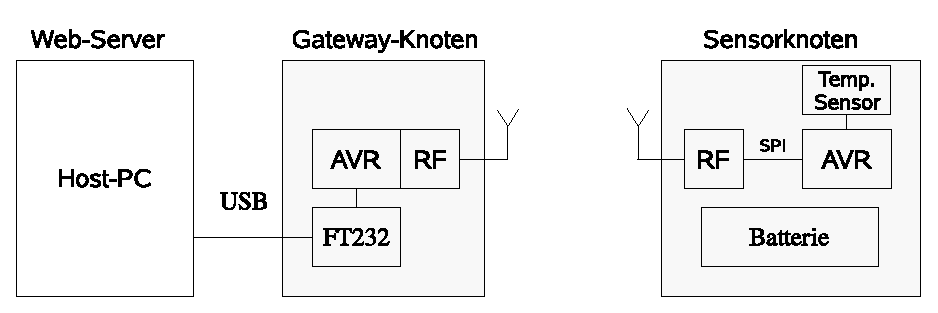
\includegraphics[width=.85\linewidth]{block1}
\caption{Blockschaltbild des Sensornetzwerks}
\label{fig:block1}
\end{figure}

Dar"uber hinaus sind {\bf Printed Circuit Boards} (PCB) verf"ugbar, die mit einem seriellen oder USB-Interface,
Steckleisten und Batteriehaltern ausger"ustet sind. Diese etwas gr"o\ss{}eren Platinen eignen sich zum
direkten Einbau in ein Ger"at. Als Beispiele seien hier
die {\em ANY-Bricks} und {\em ANY-Dongles} der \textsf{Adaptive Network Solutions GmbH},
die {\em ICRadio-Minis} und {\em ICRadio-Sticks} der \textsf{In-Circuit GmbH},
die {\em Radio Controller Boards (RCBs)} der \textsf{dresden elektronik ingenieurtechnik gmbh},
sowie der {\em AVR-Raven} und der {\em AVR-RZUSB-Stick} von \textsf{Atmel} genannt.

Ebenfalls gibt es die ersten {\bf Eigenbau-PCBs}, z.B. das {\em Muse231} vom
\textsf{Ingenieurb"uro Dietzsch und Thiele PartG}, das {\em RadioFaro-Board} von Daniel Thiele,
das {\em tiny230 Radio Board} von J"org Wunsch, sowie {\em Zigduino}
von \textsf{Logos Electromechanical LLC}.
Besonderer Augenmerk ist beim Eigenbau auf die rechtlichen Aspekte zu legen; 
dies ist bei Nutzung fertiger Module oder PCBs etwas einfacher.
% ==================================================================
\section{Ein einfaches Sensornetzwerk}
Das vorgestellte Sensornetzwerk besteht aus einem Gateway-Knoten und
einem oder mehreren Sensorknoten. Der Gateway-Knoten ist "uber eine
serielle Schnittstelle mit dem PC verbunden. Die batteriebetriebenen
Sensorknoten messen zyklisch die Temperatur und / oder andere physikalische
Gr"o\ss{}en  und senden die Messwerte zum Gateway-Knoten, der die empfangenen
Daten "uber die serielle Schnittstelle ausgibt. Von dort k"onnen sie im
PC, zum Beispiel von einem Python-Script weiterverarbeitet werden.

Am Ende des Artikels wird ein kleines Script vorgestellt, das die empfangenen
Sensordaten als HTML-Seite aufbereitet und "uber einen Webserver im Netz bereitstellt.
Das vorgestellte Beispiel soll vor allem das Konzept erkl"aren und ist nicht auf
Sicherheit optimiert.

Als {\bf Gateway-Knoten} soll hier das {\em Radifaro-Board} von Daniel Thiele
verwendet werden. Dieses Board ist kompatibel zum Arduino Duemilanove, wobei der
ATmega168 gegen ein ATmega128RFA1-Modul von \textsf{dresden elektronik} ausgetauscht
wurde. Als {\bf Sensorknoten} werden das {\em tiny231} von J"org Wunsch und das {\em Muse231}
vom \textsf{Ingenieurb"uro Dietzsch und Thiele} eingesetzt.
Beide Boards sind mit einem AT86RF231-Transceiver best"uckt,
die eingesetzten Microcontroller hingegen sind unterschiedlich, beim {\em Muse231} ist es ein ATmega88PA und beim
{\em tiny231} ein ATtiny84. Weitere Informationen zu den Boards befinden sich auf der Hompage des Vortrages.

Die n"achsten Abschnitte beschreiben die Hard- und Sofftwarevoraussetzungen
zur Programmierung der Funkmodule sowie die schrittweise Inbetriebnahme des gesamten
Systems.

\begin{figure}
\centering
\includegraphics[width=.80\linewidth]{boards}
\caption{Die verwendeten Funkknoten}
\label{fig:boards}
\end{figure}

\section{Entwicklungsumgebung}
\subsection*{Auswahl eines Programmieradapters}

Die Firmware des Microcontrollers kann mit einem Programmieradapter oder mit einem Bootloader
ge"andert werden.
Besitzt man Funkmodule mit einem vorprogrammierten Bootloader, kann man zun"achst auf die
Anschaffung eines Programmieradapters verzichten. Sp"atestens jedoch, wenn man sich durch
einen Programmierfehler aus dem Bootloader ausgesperrt hat oder die Fuses des Controllers
ge"andert werden sollen, kommt man um die Anschaffung eines Programmieradapters nicht herum.

Die Microcontroller der AVR-Familie k"onnen "uber eine 4-Drahtschnittstelle, dem sog. {\em ISP-Interface} oder
"uber das {\em JTAG-Interface} programmiert werden. Bekannte ISP-Programmier\-adapter sind u.a.
PonyProg (sp12), USBasp, \textsf{Atmel} AVR-ISP und Arduino.
Als JTAG Programmieradapter kommen \textsf{Atmel}s AVR-Dragon und JTAG-ICE MkII zum Einsatz.

Der AVR-Dragon Programmieradapter ist f"ur Bastler eine gute Wahl, da er zum einen erschwinglich
ist und zum anderen alle Programmier- und Debugmodi von AVR-Controllern unterst"utzt. Man
muss sich allerdings um ein Geh"ause und ggf. die Best"uckung einiger Stiftleisten selbst bem"uhen.

\subsection*{Installation der Software}
Die {\bf AVR-Toolchain} f"ur Linux besteht aus dem GCC-Compiler, dem GNU-Linker aus den
{\em binutils} und der AVR-libc. Der Programmieradapter wird mit dem Programm avrdude angesteuert
und das Debugging erfolgt mit AVaRICE und avr-gdb.
Unter Ubuntu erfolgt die Installation der Pakete mit dem Befehl:
\begin{lstlisting}
 > sudo apt-get install avr-libc binutils-avr gcc-avr \
                        avrdude avarice gdb-avr
\end{lstlisting}

Das {\bf $\mu{}$racoli-Projekt} stellt f"ur \textsf{Atmel} Transceiver und Microcontroller
eine Treiber-Bibliothek und Beispielanwendungen bereit. Die Software ist unter der
{\em modified BSD license} ver"offentlicht und kann somit f"ur Open- und Closed-Source-Projekte
problemlos eingesetzt werden.
Mit den bereitgestellten Funktionen kann die Funkkommunikation zwischen zwei
oder mehreren Knoten einfach implementiert werden, ohne da\ss{} man dazu vorher komplexe
Protokollregelwerke gelesen und verstanden haben mu\ss{}.
Die Pakete {\tt uracoli-src-{\em<version>}.zip} und {\tt uracoli-doc-{\em<version>}.zip} k"onnen
von \url{http://uracoli.nongnu.org/download.html} bezogen werden.

F"ur die Webserver Applikation wird sp"ater die Scriptsprache
{\bf Python} und das Modul {\bf pyserial} ben"otigt und wie folgt installiert:
\begin{lstlisting}
 > sudo apt-get install python python-serial
\end{lstlisting}

\subsection*{Anschlie"sen der Hardware}
Nach der Software-Installation kann der Gateway-Knoten an den PC
angeschlossen werden. Um die zum Board zugeh"orige serielle Schnittstelle zu
ermitteln, verwendet man den Befehl {\tt dmesg}.

\begin{lstlisting}
 > dmesg | grep tty
00:08: ttyS0 at I/O 0x3f8 (irq = 4) is a 16550A
00:09: ttyS1 at I/O 0x2f8 (irq = 3) is a 16550A
usb 2-3.3: FTDI USB Serial Device converter now attached to ttyUSB0
\end{lstlisting}

Wenn das Board mit einen USB Anschlu\ss{} ausgestattet ist, dann ist der
Ger"atename entweder {\tt /dev/ttyUSBx} oder {\tt /dev/ttyACMx}.
Die {\em STK541 USB Adapter Boards} von \textsf{Atmel} und die {\em Sensor Terminal Boards}
von \textsf{dresden elektronik} melden sich mit herstellerspezifischen Vendor und Device IDs
am Bus an und werden ab der Linux-Kernelversion 2.6.29 automatisch als
serielle Schnittstellen erkannt.

\subsection*{Einrichtung der Funkknoten}
Zun"achst wird aus dem $\mu$racoli-Paket
die Wireless-UART-Firmware {\tt wuart\_{\em<board>}.hex} auf den {\bf Gateway-Knoten} geladen. Mit diesem
Programm wird eine bidirektionale transparente Datenverbindung zwischen Funk- und UART-Interface
hergestellt. Welchen Namen man f"ur {\em<board>} einsetzt und wie die Fuses richtig programmiert
werden, entnimmt man dem Abschnitt "`Boards and Modules"' der Dokumentation.

Bei der Inbetriebnahme eines neuen Boards m"ussen zun"achst die Fuses des Controllers
richtig programmiert werden. Die Fuse-Werte stellen neben der Taktfrequenz und der
Taktquelle weitere Parameter, z.B. die Gr"o\ss{}e des Bootloaders und die Verf"ugbarkeit
von SPI- oder JTAG-Interface ein. Das Programmieren der Fuses sollte sehr sorgf"altig
erfolgen, da bei falscher Wahl der Controller u.U. nicht mehr programmierbar ist. Eine
wertvolle Hilfe bei der Fuse-Definition ist die Webanwendung Fusecalc \cite{fusecalc}.
Das Prorammieren der Fuses und der Firmware f"ur ein {\em RadioFaro}-Board "uber ein JTAG-ICE MkII
erfolgt mit den folgenden Befehlen:
\begin{lstlisting}
 > avrdude -P usb -p m128rfa1 -c jtag2 -U lfuse:w:0xff:m\
           -U hfuse:w:0xda:m -U efuse:w:0xf5:m\
 > avrdude -P usb -p m128rfa1 -c jtag2 \
           -U bin/wuart_radiofaro.hex
\end{lstlisting}

Im n"achsten Schritt wird ein Terminalprogramm auf der betreffenden Schnittstelle
ge"offnet. Anstelle vom Klassiker {\tt minicom} kann auch das Script
{\tt miniterm.py} \cite{miniterm} aus den Beispielen des pySerial-Modules verwendet werden.
Nach einem Reset des Gateway-Knotens sieht man die Startmeldung der Wireless-UART-Firmware im
Terminalfenster.
\begin{lstlisting}
 > python miniterm.py -p /dev/ttyUSB1
--- Miniterm on /dev/ttyUSB1: 9600,8,N,1 ---
--- Quit: Ctrl+]  |  Menu: Ctrl+T | Help: Ctrl+T followed by Ctrl+H ---
Wuart 0.2 chan=17
\end{lstlisting}

Ein einfaches Test-Programm {\tt xmpl\_linbuf\_tx\_{\em<board>}} f"ur den {\bf Sensorknoten} mu\ss{}
zun"achst compiliert werden. Das erfolgt
im Verzeichnis {\tt uracoli-src-{\em<version>}/xmpl} f"ur ein {\tt Muse231} Board
mit dem Befehl:
\begin{lstlisting}
 > make -f xmpl_linbuf_tx.mk muse231
\end{lstlisting}

Danach wird die Firmware {\tt bin/xmpl\_linbuf\_tx\_muse231.hex} zusammen
mit den passenden Fuse-Werten auf den Sensorknoten geladen.
Wenn nach einem Reset des Boards eine LED am Gateway-Knoten blinkt und im
Fenster des Terminalprogramms ein zyklischer Text ausgegeben wird
({\em A wonderful bird \dots}), besteht eine Funkverbindung zwischen den beiden
Knoten.

% ==================================================================
\section{Die Sensoranwendung}

Die Sensor-Anwendung erfa\ss{}t zyklisch Me\ss{}daten und sendet diese zum
Gateway-Knoten. Im Verzeichnis \texttt{Src/Sensor} befinden sich
die Firmware \texttt{bin/sensorapp\_{\em<board>}.hex}, das GNU-Makefile
\texttt{sensorapp.mk}, der C-Source-Code \texttt{sensorapp.c}, sowie das Headerfile 
\texttt{sensorapp.h}. Die Programmierung des Sensorknotens erfolgt wie oben beschrieben.

Die \texttt{main}-Funktion der Sensor-Anwendung f"uhrt die Funktion \texttt{app\_init()}
einmal aus und ruft danach in einer Endlosschleife abwechselnd \texttt{app\_task()}
und \texttt{do\_sleep()} auf.
\begin{lstlisting}[language=C]
int main(void) {
    app_init();
    timer_start(tmr_transmit, T_TX_PERIOD, 0);
    while(1) {
        app_task();
        do_sleep();
    }
}
\end{lstlisting}

Die Funktion \texttt{app\_task()} implementiert einen Zustandsautomaten, der
die Messung der Temperatur durchf"urt und das Ergebnis per Funk versendet.
Nach dem Versenden des Rahmens wird die Funktion \texttt{usr\_radio\_tx\_done()} von
der Interrupt Service Routine des Transceivers aufgerufen. In der Funktion
wird ein Timer gestartet, der seinerseits bei Ablauf das Event \texttt{APP\_MEASURE}
generiert.

\begin{lstlisting}[language=C]
void app_task(void) {
    app_event_t state;
    cli();
    state = app_event;
    app_event = APP_IDLE;
    sei();
    do {
        switch(state) {
            case APP_MEASURE:
                temp_start();
                state = APP_RESULT;
                break;
            case APP_RESULT:
                sprintf(TxFrame.data,
                        "n: 0x%04x, t: %d\n\r",
                        TxFrame.src, temp_get());
                radio_set_state(STATE_TXAUTO);
                radio_send_frame(sizeof(TxFrame),
                      (uint8_t *)&TxFrame, 0);
                state = APP_IDLE;
                break;
            default:
                state = APP_IDLE;
                break;
        }
    } while(state != APP_IDLE);
}
\end{lstlisting}

% ==================================================================
% $Id$
\section{Webserver}
%
%
"Uber die serielle Schnittstelle des Host-PCs werden nun die Daten der Sensorknoten empfangen
und es k"onnen auch Daten an diese gesendet werden. 
Als einfaches Beispiel wird hier das Auslesen und
Darstellen der von den Sensorknoten gemessenen Temperaturen mit Hilfe 
eines Webservers gezeigt. Dieser ist in Python geschrieben und verwendet
die Module \texttt{Simple\-HTTP\-Server} und \texttt{SocketServer}.
Das Server wird mit dem Befehl \texttt{python webserver.py} gestartet und 
ist danach unter \texttt{http://localhost:8080} erreichbar.

\begin{lstlisting}[tabsize=4]
import SocketServer
import SimpleHTTPServer
...
class CustomHandler(SimpleHTTPServer.SimpleHTTPRequestHandler):
    def do_GET(self):
        global sdev
        self.send_response(200)
        self.send_header('Content-type','text/html')
        self.end_headers()
        txt = sdev.build_sensor_html_table()
        self.wfile.write(header() + txt + footer())

if __name__ == "__main__":
	...
    httpd = SocketServer.ThreadingTCPServer(
                    ('localhost', PORT),CustomHandler)
	...
	httpd.serve_forever()
\end{lstlisting}

In einem separaten Thread werden die ankommenden Sensordaten von der
seriellen Schnittstelle gelesen und in einem Dictionary gespeichert.
Die Funktion {\tt build\_sensor\_html\_table()} baut daraus eine HTML-Tabelle. 
Diese Methode wird von der oben beschriebenen Serverfunktion 
{\tt do\_GET()} aus aufgerufen.
\begin{lstlisting}[tabsize=4]
class Device:
    def __init__(self,port, baud, verbose=0):
        self.sport = serial.Serial(port, baud)
        self.rxThread = threading.Thread(target = self._rx_thread_)
        ...
        self.rxThread.start()
        self.sensor_data = {} # collects sensor data

    # function running in thread
    def _rx_thread_(self):
        while 1:
            sline = self.sport.readline().strip()
            tim = int(time.time())
            (node, temp) = self.parse_line(sline)
            self.sensor_data[node] = (tim, temp)

    def build_sensor_html_table(self):
        ...
        for node in nodes:
            ...
            (tim,temp) = self.sensor_data[node]
            if (int(time.time()) - tim) > 10:
                ret += '<td style="color:red">'\
                       '%s</td>\n' % temp
            else:  
                ret += '<td>%s</td>\n' % temp
        ...
        return ret
\end{lstlisting}


% ==================================================================
\section{Ausblick}
Im Artikel wurde die Einrichtung und Inbetriebnahme einer Entwicklungsumgebung
f"ur \textsf{Atmel}-basierte IEEE-802.15.4 Funkmodule beschrieben. Mit der verf"ugbaren
Open-Source-Soft\-ware ist es m"oglich, einfache kleine Sensornetzwerke
aufzubauen. Die gezeigten Beispiele sollen als Anregung dienen und Lust auf
eigene Experimente machen. "Uber Anregungen, Fragen und aktive Hilfe freut
sich das $\mu{}$racoli-Team.

% ==================================================================

\begin{thebibliography}{XX}
\bibitem{ism}
    \emph{ISM-Band}. Wikipedia\\
    \url{http://de.wikipedia.org/wiki/ISM-Band}
\bibitem{ieee154}
    \emph{IEEE 802.15 Standards}. IEEE\\
    \url{http://standards.ieee.org/about/get/802/802.15.html}
\bibitem{uracoli}
    \emph{$\mu{}$racoli - The Micro Controller Radio Communication Library}. Homepage\\
    \url{http://uracoli.nongnu.org}
\bibitem{miniterm}
    \emph{Examples}. pySerial v2.5 Documentation\\
    \url{http://pyserial.sourceforge.net/examples.html}
\bibitem{fusecalc}
    \emph{Engbedded Atmel AVR Fuse Calculator}. Mark H"ammerling\\
    \url{http://www.engbedded.com/fusecalc}
\end{thebibliography}
\end{document}
